\documentclass[12pt]{article}

\usepackage{graphicx}
\usepackage{amsmath}
\usepackage{amssymb}
\usepackage{natbib}
\usepackage{amsfonts}
\usepackage{multicol}
\usepackage{float}
\usepackage{oldgerm}
\usepackage{bm}
\usepackage{mathtools}
\usepackage{wrapfig}
\usepackage{fancyhdr}
\usepackage[export]{adjustbox}
\usepackage{xcolor}

\pagestyle{empty}

\newcommand{\avec}{{\mathbf A}}
\newcommand{\bvec}{\mathbf B}
\newcommand{\dvec}{\mathbf D}
\newcommand{\evec}{\mathbf E}
\newcommand{\fvec}{\mathbf F}
\newcommand{\jvec}{\mathbf J}
\newcommand{\kvec}{{\mathbf {k}}}
\newcommand{\mvec}{{\mathbf {M}}}
\newcommand{\nbold}{{\mathbf n}}
\newcommand{\vvec}{\mathbf{v}}
\newcommand{\xvec}{{\mathbf x}}
\newcommand{\yvec}{{\mathbf y}}
\newcommand{\zvec}{{\mathbf z}}
\newcommand{\nablav}{\boldsymbol{\nabla}}
\newcommand{\phivec}{\boldsymbol{\phi}}
\newcommand{\epvec}{\boldsymbol{\epsilon}}
\newcommand{\ezero}{\epsilon_{0}}
\newcommand{\mzero}{\mu_{0}}
\newcommand{\mubold}{\boldsymbol{\mu}}
\newcommand{\uniti}{\hat{\boldsymbol{\imath}}}
\newcommand{\unitj}{\hat{\boldsymbol{\jmath}}}
\newcommand{\unitk}{\hat{\boldsymbol{\mathit{k}}}}
\newcommand{\unitn}{\hat{\mathbf n}}
\newcommand{\unitr}{\hat{\mathbf r}}
\newcommand{\unitphi}{\boldsymbol{\phi}}
\newcommand{\unittheta}{\boldsymbol{\theta}}

\newcommand{\bit}{\begin{itemize}}
\newcommand{\eit}{\end{itemize}}

\setlength{\headsep}{0.5cm}
\setlength{\oddsidemargin}{-0.5cm}
\setlength{\textwidth}{16.5cm}
\setlength{\textheight}{24cm}
\voffset = -2cm

\pagestyle{fancy}
\fancyhf{}
\rfoot{
\includegraphics[width=1.0in]{cnm.png}}
\lfoot{Quiz 2}

\begin{document}

%{\bf \underline{STUDENT NAME}:} 
%\vspace{1cm}

\begin{center}
%\date{10/02/18-10/09/18}
\hfil
{\large\bf {ENGR 2910: Circuit Analysis I}}
\hfill Instructor: Leo Silbert \\
Quiz 2: Monday, Sept. 13\\
\hrulefill\\
\end{center}

%{\em Show all your working to ensure you obtain full points. Partial
%  credit will be given for correct algebraic steps if you fail to
%  obtain the correct final answer.}\\

%\newpage


\noindent
\noindent
{\bf Question 1} [2]

Label each of the sources below indicating whether they are voltage or current sources, and whether they are independent or dependent sources.
\begin{figure}[h!]
\centering
(a)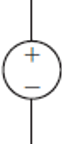
\includegraphics[width=0.5in]{Source1.png}
(b)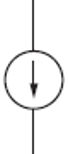
\includegraphics[width=0.5in]{Source2.png}
(c)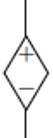
\includegraphics[width=0.5in]{Source3.png}
(d)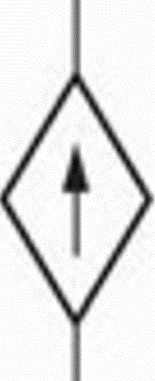
\includegraphics[width=0.5in]{Source4.jpg}
\end{figure}

\vspace{2.0in}
\noindent
{\bf Question 2} [4]

Which of the following circuits are valid?
\begin{figure}[h!]
\centering
(a)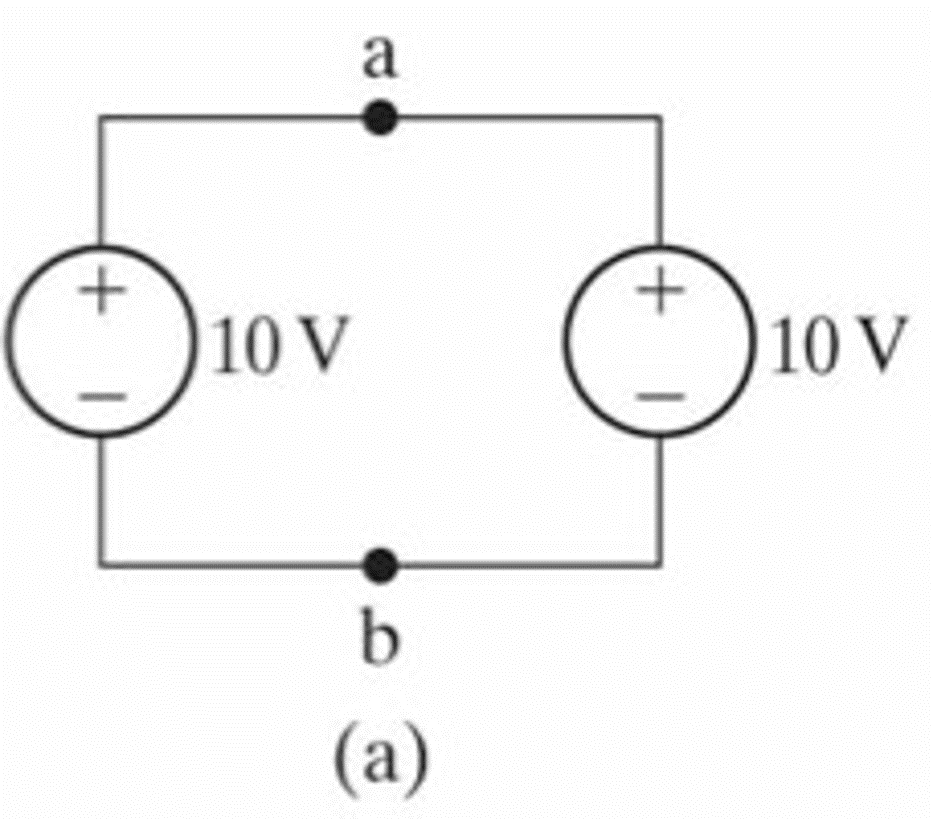
\includegraphics[width=1.0in]{Good1.png}
(b)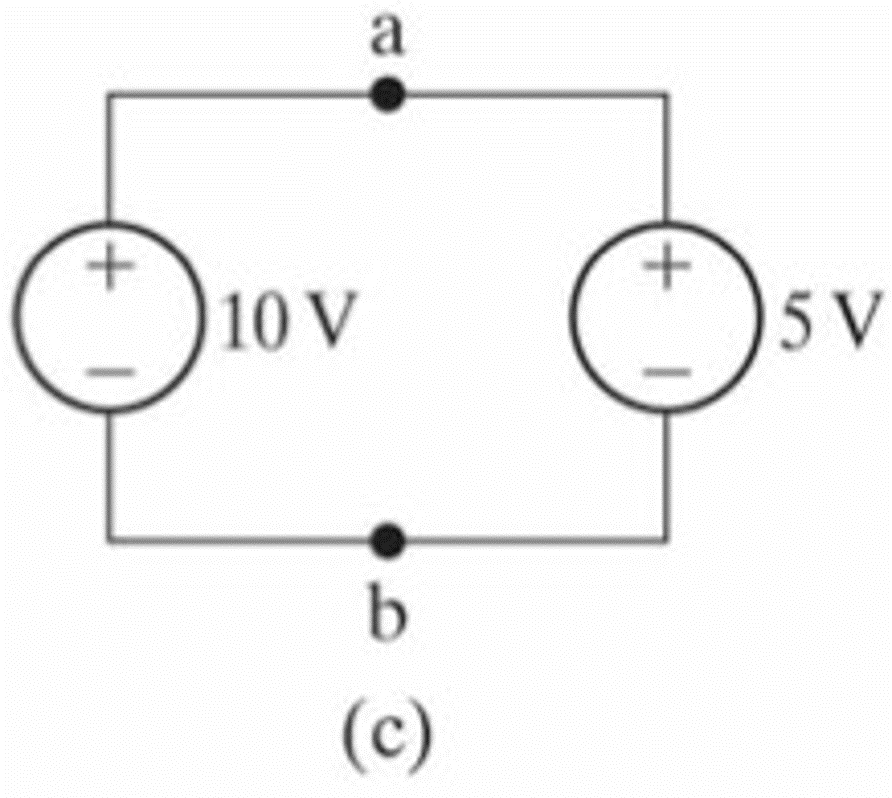
\includegraphics[width=1.0in]{Bad1.png}
(c)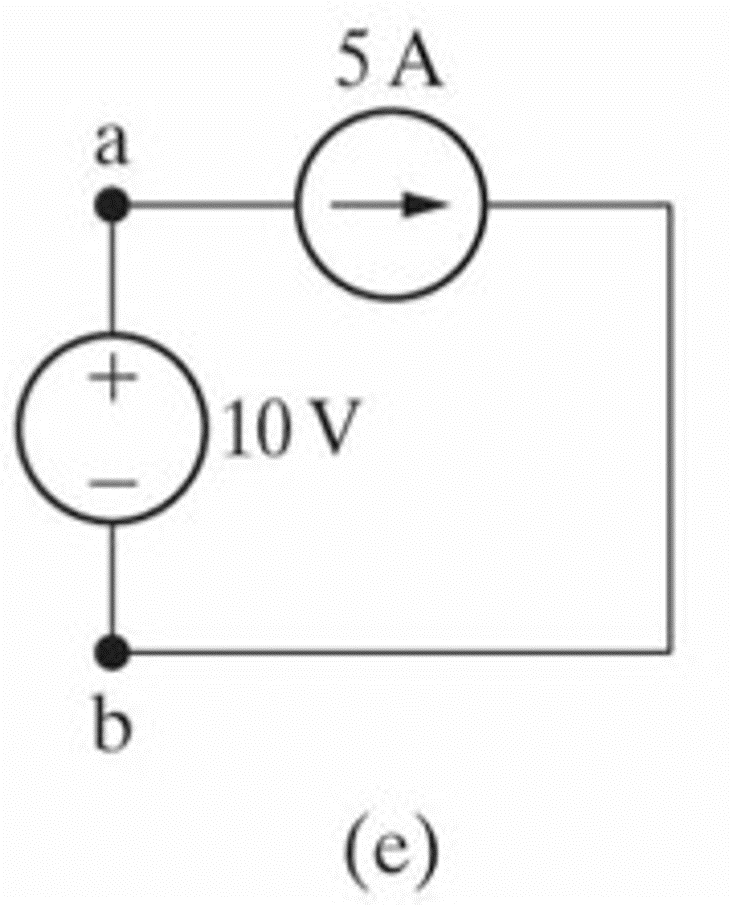
\includegraphics[width=1.0in]{Good2.png}
(d)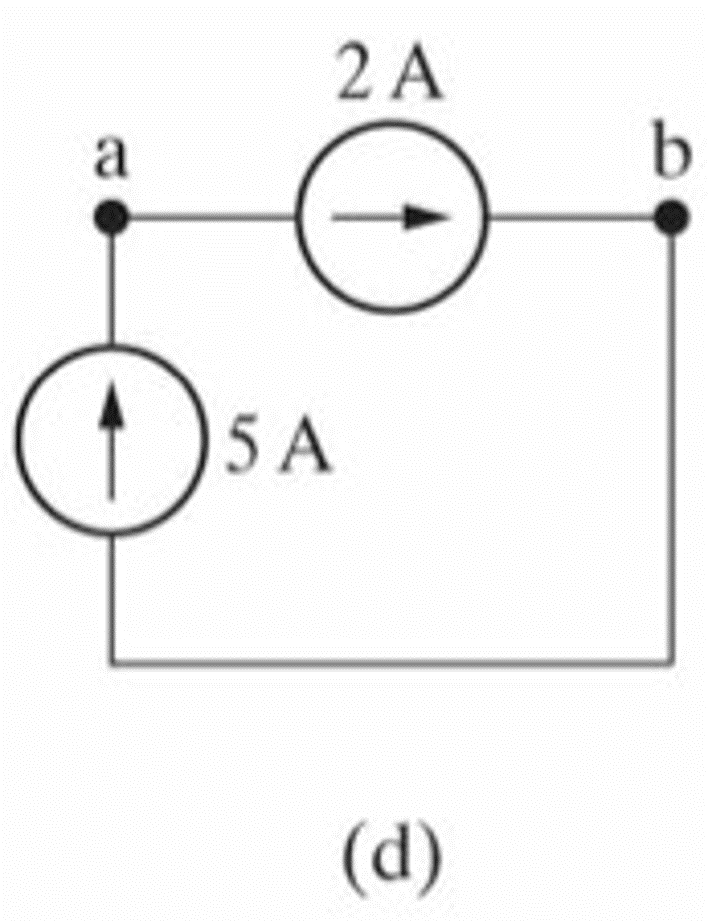
\includegraphics[width=1.0in]{Bad2.png}
\end{figure}

\newpage
\noindent
{\bf Question 3} [2]

Write down and explain Ohm's Law.

\vspace{2.0in}
\noindent
{\bf Question 4} [2]

Write down and explain Kirchoff's Laws.


\end{document}
